\section{一元函数的连续性和微分}
\label{sec:analysis-local-models}

设$f:I\to\mathbb R$，其中$I$是实轴上的区间。输入$x$趋近$a$时，函数值是否趋近$f(a)$，这是连续性的问题；
函数增量能否由一个关于输入增量的线性式近似，这是可微性的问题。
第~\ref{sec:analysis-function-limits}节的函数极限已经说明了“输入趋近时输出趋向何处”，
第~\ref{sec:analysis-metric-measurement}节又给出了开集、闭集与紧致性。

本节先用函数极限定义连续性，比较几种强弱不同的连续性条件，并在比较时证明一致连续性定理，利用连续性研究闭区间上的最值与介值。
随后用差商的极限定义导数，把它改写为线性近似，得到求导规则；
最后用中值定理和Taylor公式，把一点处的导数信息转化为对有限区间上函数变化的控制。

\subsection{连续函数}
\label{sec:analysis-metric-continuity-extrema}

\subsubsection{连续性}

\paragraph{连续函数}
对$f(x)=x^2$，当$x$接近$a$时，$f(x)$接近$a^2=f(a)$，这正是连续性要表达的关系。下面用邻近输入的误差条件规定连续性，定义域也可以不是整个区间。
\begin{definition}[连续函数]
\label{def:analysis-continuity}
设$X\subseteq\mathbb R$，$a\in X$。若对每个$\varepsilon>0$，都存在$\delta>0$，使
\[
 x\in X,\quad |x-a|<\delta
 \quad\Longrightarrow\quad |f(x)-f(a)|<\varepsilon,
\]
则称$f:X\to\mathbb R$在$a$处\term{连续}（continuous）。若$f$在$X$的每一点连续，就称$f$为连续函数。
\end{definition}
这里$\delta$可以依赖$a$和$\varepsilon$。若$a$是$X$的聚点，定义等价于$\lim_{x\to a,\,x\in X}f(x)=f(a)$；若$a$是孤立点，取足够小的$\delta$使邻域内只有$a$，定义自动成立。在闭区间端点处，只取定义域内的输入，因而连续性分别用右极限或左极限判断。

例如在$|x-a|<1$时，$|x^2-a^2|\leq(2|a|+1)|x-a|$。给定$\varepsilon>0$，取$\delta=\min\{1,\varepsilon/(2|a|+1)\}$即可验证平方函数在每个$a$处连续。

\paragraph{度量下的连续性}
前面的定义使用绝对值距离；第~\ref{sec:analysis-set-metric}节已经将距离推广到一般集合，连续性也可以作同样的推广。
设$(X,d_X)$、$(Y,d_Y)$为度量空间，$f:X\to Y$，$a\in X$。$f$在$a$处连续，是指
\[
 \forall\varepsilon>0,\quad\exists\delta>0,\quad\forall x\in X,\qquad
 d_X(x,a)<\delta\Longrightarrow d_Y(f(x),f(a))<\varepsilon.
\]
输入距离控制输出距离，分别替代原定义中的两个绝对值；取实轴上的通常距离便回到一元实函数的定义。
这里包含$x=a$，因而不要求$a$为聚点；在所选度量下孤立的输入点处，函数自动连续。改变距离可能改变连续性。例如恒等映射从实轴通常距离映到离散距离时不连续，因为不同输出的距离始终为$1$；反向的恒等映射则连续，因为输入距离小于$1$时两点已经相同。图~\ref{fig:analysis-metric-convergence}同时比较这两种距离下的序列收敛与连续性。
\begin{figure*}[htbp]
 \centering
 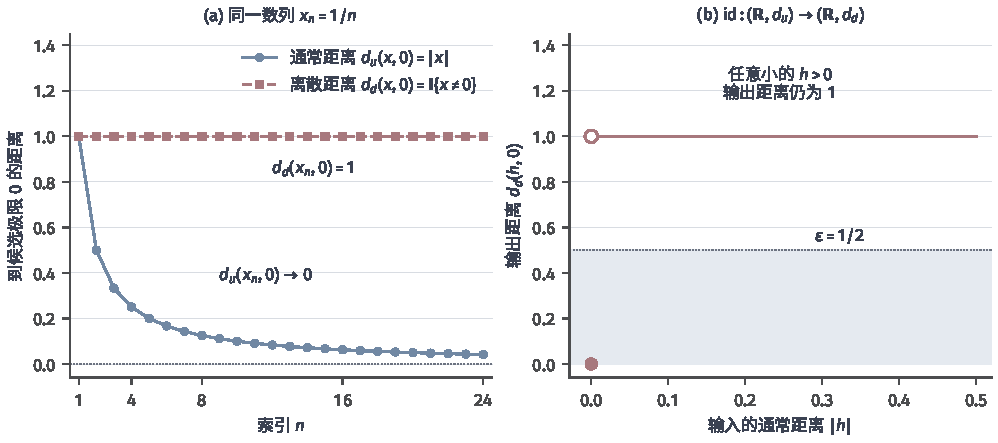
\includegraphics[width=169.0mm]{figures/01-mathematical-preliminaries-upper/01-mathematical-language-combinatorics-analysis-optimization/matplotlib/analysis-metric-convergence/figure.pdf}
 \caption{通常距离与离散距离给出的不同邻近关系，图中分别记为$d_u$和$d_d$。左图中$1/n$在通常距离下趋于$0$，在离散距离下与$0$的距离始终为$1$；右图比较恒等映射的连续性。实轴上的通常距离是本节一元连续性与微分的默认距离。}
 \label{fig:analysis-metric-convergence}
\end{figure*}

\paragraph{连续性的序列判据}
连续性除了用邻域误差检验，也可以通过趋近点列来检验，后者便于回用已经建立的数列结论。
连续性等价于：对任意满足$x_n\in X$、$x_n\to a$的序列，都有$f(x_n)\to f(a)$。连续时，将定义用于序列的尾部就得到这一结论。反之，若连续性不成立，就存在$\varepsilon_0>0$，使每个$1/n$邻域内都能选到$x_n\in X$，满足$|f(x_n)-f(a)|\geq\varepsilon_0$；此时$x_n\to a$而函数值不趋于$f(a)$。

\paragraph{间断点}
连续性失效可能来自极限不存在，也可能只是极限与点值不一致，需要按这些不同情形说明间断。
函数在定义域的一点不连续，就称该点为间断点。若有限极限存在而不等于点值，称为可去间断；若左右有限极限存在但不同，称为跳跃间断。例如将$x^2$在$0$处的值改为$1$，就在$0$处产生可去间断；阶跃函数$\mathbb I\{x\geq0\}$在$0$处左右极限分别为$0$和$1$。这些名称描述不同的失效方式，并未穷尽所有间断情形。

\subsubsection{连续函数的运算}

连续性已经把函数值与输入极限联系起来。固定有限个连续函数进行运算，可以直接回用函数极限的运算法则。
下面的极限公式先针对定义域的聚点$a$；若$a$为孤立点，所有在该点有定义的组合函数都直接由连续定义满足连续性。

\paragraph{和的连续性}
把两个连续函数相加，输入趋近时，两项分别趋于各自的点值，因而和也趋于点值之和。
若$f,g:X\to\mathbb R$在$a\in X$处连续，则
\[
 \lim_{x\to a}(f(x)+g(x))=f(a)+g(a)=(f+g)(a),
\]
所以$f+g$在$a$处连续。这里及以下极限均沿定义域$X$取。

\paragraph{差的连续性}
相减时分别控制两项的误差，仍能控制结果的误差。若$f,g$在$a$处连续，则
\[
 \lim_{x\to a}(f(x)-g(x))=f(a)-g(a)=(f-g)(a),
\]
所以$f-g$在$a$处连续；这也可直接由差的极限法则得到。

\paragraph{数乘的连续性}
固定实常数$c$只把输出误差乘以$|c|$。若$f$在$a$处连续，则
\[
 \lim_{x\to a}cf(x)=cf(a),
\]
所以$cf$在$a$处连续，$c=0$时所得常函数同样连续。

\paragraph{积的连续性}
乘积可以使用积的极限法则，因为两个因子在$a$附近都具有有限极限。
若$f,g$在$a$处连续，则
\[
 \lim_{x\to a}f(x)g(x)=f(a)g(a)=(fg)(a),
\]
所以$fg$在$a$处连续。

\paragraph{商的连续性}
除法还要防止分母在基点附近变为零。若$f,g$在$a$处连续且$g(a)\neq0$，
由$g$的连续性可取$a$的一个相对邻域，使其中$|g(x)|>|g(a)|/2$，于是
\[
 \lim_{x\to a}\frac{f(x)}{g(x)}=\frac{f(a)}{g(a)}.
\]
因此$f/g$在$a$附近有定义，并在$a$处连续；分母非零的条件不能省略。

\paragraph{复合函数的连续性}
复合要求内层函数的输出能够作为外层函数的输入，因此两层的定义域必须衔接。
设$f:X\to Y$在$a\in X$处连续，$g:Y\to\mathbb R$在$f(a)$处连续，其中$X,Y\subseteq\mathbb R$，则$g\circ f$在$a$处连续。
给定$\varepsilon>0$，先由$g$的连续性取$\eta>0$，使$y\in Y$且$|y-f(a)|<\eta$时$|g(y)-g(f(a))|<\varepsilon$；
再由$f$的连续性取$\delta>0$，使$x\in X$且$|x-a|<\delta$时$|f(x)-f(a)|<\eta$。两步合并便得到复合函数的连续性。

\paragraph{反函数的连续性}
\label{sec:analysis-inverse-continuity}
严格单调性给出逆映射后，还需确认像点的小扰动不会使反像突然跳动。
若$f$在区间$I$上连续且严格单调，它是一一对应于像集$f(I)$的函数，反函数在$f(I)$上连续。以严格递增为例，固定内点$a\in I$，在$a$两侧选$a-\varepsilon,a+\varepsilon\in I$；它们的函数值严格夹住$f(a)$，因此充分接近$f(a)$的像点，其反像必落在这两个点之间。端点只保留存在的一侧，同样得到相对定义域的连续性。

\subsubsection{连续性条件及其关系}
\label{sec:analysis-continuity-relations}

逐点连续允许每个基点使用不同的误差尺度；对整个范围共同控制输入误差，或同时控制许多小区间的总变化，就得到下面几种不同的要求。

\paragraph{一致连续函数}
平方函数在每一点连续，但定义中的$\delta$会随$a$的位置改变。若要用同一个输入误差控制定义域内所有位置，就需要更强的条件。
\begin{definition}[一致连续函数]
\label{def:analysis-uniform-continuity}
函数$f:X\to\mathbb R$称为\term{一致连续}（uniformly continuous），若对每个$\varepsilon>0$，都存在$\delta>0$，使任意$x,y\in X$满足
\[
 |x-y|<\delta\quad\Longrightarrow\quad |f(x)-f(y)|<\varepsilon.
\]
\end{definition}
$\delta$只依赖$\varepsilon$，不再依赖所选的$x,y$。平方函数在$\mathbb R$上不一致连续：取$x_n=n$、$y_n=n+1/n$，输入距离趋于零，输出之差却为$2+1/n^2$。若它一致连续，取固定的输出误差$1$就会与这两列点矛盾。

\paragraph{Lipschitz连续函数}
一致连续只要求某个共同的$\delta$存在；有些函数还能用输入距离的常数倍控制输出距离。
\begin{definition}[Lipschitz连续函数]
\label{def:analysis-lipschitz-continuity}
函数$f:X\to\mathbb R$若存在有限常数$L\geq0$，使所有$x,y\in X$都满足
\begin{equation}
 |f(x)-f(y)|\leq L|x-y|,
\label{eq:analysis-lipschitz-condition}
\end{equation}
则称$f$为\term{Lipschitz连续}（Lipschitz continuous）函数，$L$称为一个Lipschitz常数。
\end{definition}
在$[0,1]$上，$|x^2-y^2|\leq2|x-y|$，所以平方函数可取$L=2$。这种线性误差界与其他连续性条件的关系，将在本小节各项定义齐备后统一证明。

\paragraph{局部Lipschitz连续函数}
平方函数在整个实轴上没有共同的有限Lipschitz常数，但在每个点附近都能找到这样的常数。若只研究局部变化，可以让邻域及常数随基点改变。

\begin{definition}[局部Lipschitz连续函数]
\label{def:analysis-local-lipschitz}
设$U\subseteq\mathbb R$为开集，$f:U\to\mathbb R$。若对每个$a\in U$，都存在$r>0$及有限$L\geq0$，使$(a-r,a+r)\subseteq U$，且该区间内的任意$x,y$满足式~\eqref{eq:analysis-lipschitz-condition}，则称$f$为$U$上的\term{局部Lipschitz函数}（locally Lipschitz function）。
\end{definition}
这里的$r,L$可以随$a$改变。平方函数在$(a-r,a+r)$内可取$L=2(|a|+r)$，因此在实轴上局部Lipschitz连续，尽管没有适用于整条实轴的Lipschitz常数。

\paragraph{绝对连续函数}
一致连续控制一个短区间两端的变化；如果同时考察许多互不重叠的小区间，还可以要求总长度很小时，全部端点变化的绝对值之和也很小。这个要求称为绝对连续，它直接用区间增量定义，尚不涉及导数或积分。
\begin{definition}[绝对连续函数]
\label{def:measurable-absolutely-continuous-function}
函数$F:[a,b]\to\mathbb R$称为\term{绝对连续函数}（absolutely continuous function），若对每个$\varepsilon>0$都存在$\delta>0$，使任意有限个内部两两不交的子区间$[a_j,b_j]\subseteq[a,b]$满足
\[
 \sum_j(b_j-a_j)<\delta
 \quad\Longrightarrow\quad
 \sum_j|F(b_j)-F(a_j)|<\varepsilon.
\]
\end{definition}
例如，$\sqrt x$在$[0,1]$上的绝对连续性可直接用区间增量验证：在$\eta>0$处分开所有小区间，靠近零点的变化总和不超过$\sqrt\eta$，其余部分利用$\sqrt v-\sqrt u=(v-u)/(\sqrt v+\sqrt u)\leq(v-u)/(2\sqrt\eta)$，估计为总长度乘$1/(2\sqrt\eta)$；先选$\eta$，再限制总长度即可。这里绝对连续约束函数的区间增量，与两个测度之间同名的绝对连续关系有不同的定义对象。

四种定义已经给出，现在比较它们对同一个函数增加了哪些要求。绝对连续在这里以实数闭区间上的增量定义，所以下面的四者比较固定在同一个非退化闭区间上；一致连续性定理则先对更一般的闭有界实数集合陈述。

\paragraph{一致连续性定理}
实轴上的平方函数表明，逐点连续未必给出全域共同的误差尺度。
闭且有界的定义域则能从任意点列中取得域内收敛子列，使逐点控制合并为共同控制。
\begin{theorem}[闭有界集上的一致连续性]
\label{thm:analysis-uniform-continuity}
设$K\subseteq\mathbb R$非空、闭且有界，$f:K\to\mathbb R$连续，则$f$在$K$上一致连续，即
\[
 \forall\varepsilon>0,\quad\exists\delta>0,\quad\forall x,y\in K,\qquad
 |x-y|<\delta\Longrightarrow |f(x)-f(y)|<\varepsilon.
\]
特别地，每个闭区间上的连续函数都一致连续。
\end{theorem}
\begin{proof}
若结论不成立，存在$\varepsilon_0>0$，使每个$\delta>0$都能找到$x,y\in K$满足
$|x-y|<\delta$而$|f(x)-f(y)|\geq\varepsilon_0$。
依次取$\delta=1/n$，得到$x_n,y_n\in K$。由Bolzano--Weierstrass定理~\ref{thm:analysis-bounded-subsequence}，可选
$x_{n_k}\to x$；由闭性及闭集的序列判据，$x\in K$。
又有$|y_{n_k}-x|\leq|y_{n_k}-x_{n_k}|+|x_{n_k}-x|\to0$，所以$y_{n_k}\to x$。
连续性使$f(x_{n_k})$与$f(y_{n_k})$都趋于$f(x)$，两者之差趋零，
与始终至少为$\varepsilon_0$矛盾。
\end{proof}
这一定理不需要微分或积分；例如$\sqrt x$在$[0,1]$上连续，因而在那里一致连续。
闭、有界的条件是这里的充分保证，不能用这个定理处理整个实轴上的平方函数。

\paragraph{闭区间上的蕴含关系}
逐点控制、共同误差尺度、区间总变化与线性误差界，是四种不同要求。
定义~\ref{def:analysis-continuity}、\ref{def:analysis-uniform-continuity}、\ref{def:analysis-lipschitz-continuity}及\ref{def:measurable-absolutely-continuous-function}给出如下关系。
\begin{theorem}[闭区间上连续性条件的关系]
\label{thm:analysis-continuity-implications}
设$a<b$，$f:[a,b]\to\mathbb R$。对同一个$f$和同一个定义域，有
\[
 \text{Lipschitz连续}\ \Longrightarrow\ \text{绝对连续}
 \ \Longrightarrow\ \text{一致连续}\ \Longleftrightarrow\ \text{连续}.
\]
前两个箭头的逆向一般不成立。末尾的等价使用了定义域为闭有界区间的条件。
\end{theorem}
\begin{proof}
若$f$有Lipschitz常数$L$，对任意有限个内部两两不交的子区间，有
\[
 \sum_j|f(b_j)-f(a_j)|\leq L\sum_j(b_j-a_j).
\]
当$L>0$时取总长度小于$\varepsilon/L$，就满足绝对连续的要求；$L=0$时直接成立。
绝对连续定义只取一个子区间，就得到对所有端点通用的连续控制，因而一致连续。
一致连续的同一个$\delta$适用于每个固定基点，所以推出连续；反向由闭有界集上的一致连续性定理~\ref{thm:analysis-uniform-continuity}保证。
\end{proof}

\paragraph{逆向关系与定义域的作用}
前面直接用区间增量验证了$\sqrt x$在$[0,1]$上绝对连续，而零点附近的割线斜率$1/\sqrt x$无界，所以绝对连续不保证Lipschitz连续。
一致连续也不保证绝对连续：第~\ref{sec:analysis-cantor-function}节将构造康托尔函数，并用总长度趋零、端点变化总和却恒为$1$的区间族证明这一点。
这个反例区分了控制每一个短区间与控制许多短区间的总变化；此处先保留这一区别，完整构造及验证放在该节。

连续与一致连续的等价依赖定义域。前面实轴上的平方函数反例中，$|x_n-y_n|\to0$而$|f(x_n)-f(y_n)|\to2$；同一个表达式限制到$[0,1]$后却有Lipschitz常数$2$。
因此性质必须连同定义域一起比较。多元输入的紧集上也有连续与一致连续的等价关系，后面会证明；一元绝对连续的区间增量定义则不能直接搬到任意多元集合上。

连续性保证输入趋近时输出趋近；一致连续为整个定义域提供共同误差尺度；Lipschitz条件进一步提供线性误差上界。
绝对连续控制许多短区间的总变化，后面的微积分基本定理将说明它为何恰好适合用可积导数恢复函数。

图~\ref{fig:analysis-continuity-conditions}把这些条件放回具体函数与定义域中比较。
先比较同一个平方函数：实轴上只有局部Lipschitz控制，在$[0,1]$上却有共同常数$L=2$；
再看平方根和康托尔函数，分别区分绝对连续与Lipschitz连续、一致连续与绝对连续。
康托尔函数的定义与反例证明将在第~\ref{sec:analysis-cantor-function}节给出，这里先用图示标出需要区分的条件。
\begin{figure*}[htbp]
 \centering
 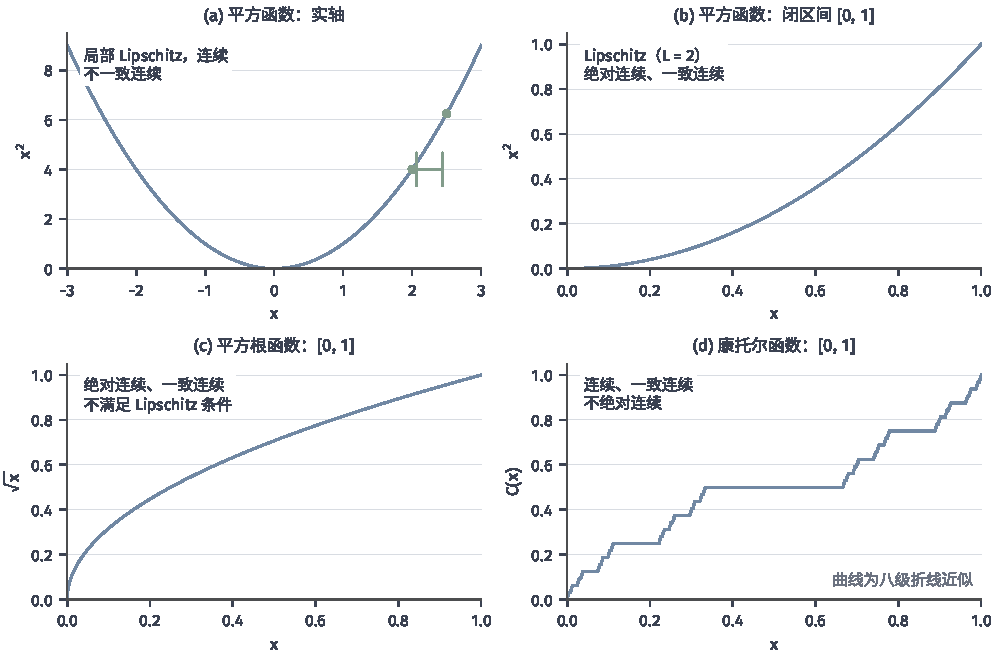
\includegraphics[width=169mm]{figures/01-mathematical-preliminaries-upper/01-mathematical-language-combinatorics-analysis-optimization/matplotlib/continuity-conditions/figure.pdf}
 \caption{连续性条件依赖于函数和定义域。(a)平方函数在实轴上连续且局部Lipschitz，但不一致连续；只展示$[-3,3]$内的曲线，标记对应$x_2=2$、$y_2=2+1/2$，完整反例使用前文的两列输入。(b)同一函数限制到$[0,1]$后为Lipschitz函数，因而绝对连续且一致连续。(c)$\sqrt x$在$[0,1]$上绝对连续、一致连续，却不是Lipschitz函数。(d)康托尔函数在$[0,1]$上连续且一致连续，但不绝对连续。右下曲线为八级折线近似，性质标注属于极限函数；每条有限折线本身都是Lipschitz函数，图形不能代替不绝对连续的证明。}
 \label{fig:analysis-continuity-conditions}
\end{figure*}

\subsubsection{闭区间上连续函数的性质}

\paragraph{有界性与最值}
第~\ref{chap:sets-functions-and-proofs}章的例子说明，函数的下确界未必取得，例如$x$在$(0,1)$上没有最小值。
寻找最小值之前，我们希望知道在什么条件下最值一定存在。
闭区间$[a,b]$中的每个序列都有收敛到区间内某点的子列：Bolzano--Weierstrass定理~\ref{thm:analysis-bounded-subsequence}给出收敛子列，
闭集的序列判据（引理~\ref{lem:analysis-closed-sequence-criterion}）保证极限仍在区间内。
结合连续性，这一事实保证函数有界并达到最值。
\begin{theorem}[闭有界集上的极值定理]
\label{thm:analysis-extreme-value}
设$K\subseteq\mathbb R$非空、闭且有界，$f:K\to\mathbb R$连续，则$f$有界，且在$K$上达到最小值和最大值。特别地，结论适用于非空闭区间。
\end{theorem}
\begin{proof}
若$f$无界，可选$x_n\in K$使$|f(x_n)|>n$。有界序列有收敛子列$x_{n_k}\to x$，闭性保证$x\in K$；连续性给出$f(x_{n_k})\to f(x)$，与$|f(x_{n_k})|>n_k$矛盾。令$m=\inf_K f$，对每个$n$选$x_n\in K$使$m\leq f(x_n)<m+1/n$。再取收敛子列$x_{n_k}\to x^\star\in K$，得到$f(x^\star)=m$。对$-f$重复论证即得最大值。
\end{proof}
\begin{example}[极值定理的条件]
\label{ex:analysis-extrema-failures}
在$(0,1)$上，连续函数$f(x)=x$的下确界为$0$却不达到，因为定义域不含边界点$0$。在闭但无界的实轴上，$e^x$也有未达到的下确界$0$。若在$[0,1]$上令$f(0)=1$、$f(x)=x$（$x>0$），定义域闭且有界，但函数不连续，同样没有最小值。
\end{example}

\paragraph{介值定理}
闭区间上的连续性还保证：函数从一个端点值变化到另一个端点值时，不会遗漏它们之间的数值。
这一结论要求两端之间的整段都在定义域中，条件比前面只要求闭且有界更具体。
\begin{theorem}[介值定理]
\label{thm:analysis-intermediate-value}
设$a,b\in\mathbb R$、$a<b$，$f:[a,b]\to\mathbb R$连续。则
\[
 \begin{gathered}
 \forall c\in[\min\{f(a),f(b)\},\max\{f(a),f(b)\}],\\
 \exists\xi\in[a,b],\quad f(\xi)=c.
 \end{gathered}
\]
若$\min\{f(a),f(b)\}<c<\max\{f(a),f(b)\}$，则可取$\xi\in(a,b)$。
\end{theorem}
\begin{proof}
$c=f(a)$或$c=f(b)$时，直接取相应端点。先设$f(a)<c<f(b)$，令
$S=\{x\in[a,b]:f(x)\leq c\}$。因$a\in S$且$S$有上界$b$，实数的确界性质给出$u=\sup S\in[a,b]$。
对每个正整数$n$，可选$x_n\in S$满足$u-1/n<x_n\leq u$，于是$x_n\to u$。
连续性使$f(x_n)\to f(u)$；由$f(x_n)\leq c$得到$f(u)\leq c$。
这也说明$u\neq b$，因为$f(b)>c$。
若$f(u)<c$，连续性保证$u$右侧充分近的点仍有函数值小于$c$；
由于$u<b$，可在$[a,b]$内选到这样的$v>u$。于是$v\in S$，与$u$为上界矛盾。
因此$f(u)=c$。又因$f(a)<c$，有$u\neq a$，所以$u\in(a,b)$。
若$f(a)>c>f(b)$，对$-f$与$-c$应用同一论证即可。
\end{proof}
介值性使用了整个区间都属于定义域。在$[-2,-1]\cup[1,2]$上，左段恒为$0$、右段恒为$1$的函数连续，却不取中间值$1/2$。
闭且有界足以保证最值，不能代替介值定理中的区间条件。

\paragraph{紧致集上的结论}
定义~\ref{def:analysis-compactness}已用开覆盖与有限子覆盖规定紧致性，并说明度量空间中的紧致性与序列紧致性的关系。
第~\ref{sec:analysis-metric-measurement}节已证明，实轴上闭且有界的集合都是紧致集。上面的极值证明与一致连续证明实际使用的，正是每个序列都能取到收敛于集合内部的子列；因此它们也适用于一般度量空间的非空紧致集。这里的一元闭有界集满足这一条件，介值结论则另外依赖定义域是区间。

\par\Needspace{10\baselineskip}
\subsection{微分的定义}
\label{sec:analysis-derivatives-linear-approximation}

连续性描述输入接近时函数值是否接近，还没有记录变化的快慢。下面先用差商的极限定义导数，再把它改写为函数增量的一阶线性近似，由此定义微分。

\subsubsection{导数}

\paragraph{差商}
设$f$在$a$的某个开区间内有定义。输入从$a$变成$a+h$时，函数增量为$\Delta f=f(a+h)-f(a)$。当$h\neq0$，比值$\Delta f/h$称为差商，表示这两个输入之间的平均变化率；在图形上，它是连接两点的割线斜率。

\paragraph{导数}
若差商在$h\to0$时趋于一个有限实数，就定义
\[
 f'(a)=\lim_{h\to0}\frac{f(a+h)-f(a)}h,
\]
称其为$f$在$a$处的\term{导数}（derivative），并称$f$在$a$处可导。导数给出该点的瞬时变化率，也是图形在该点的切线斜率。若区间内每点都可导，则$a\mapsto f'(a)$又构成一个函数，称为导函数。例如$f(x)=x^2$时，差商为$2a+h$，故$f'(a)=2a$。

\paragraph{单侧导数}
在区间端点或尖点附近，左右两侧的变化需要分别观察。
只从$h>0$或$h<0$取极限，分别得到右导数$f'_+(a)$和左导数$f'_-(a)$。内点处的双侧导数存在，当且仅当左右导数都存在、有限并且相等。在闭区间端点讨论导数时，将明确采用从区间内部取得的单侧导数。本节未特别说明的内点导数均指有限的双侧导数。

\subsubsection{可微函数}

\paragraph{可微与微分}

差商趋于$f'(a)$等价于把增量写为
\begin{equation}
 f(a+h)=f(a)+f'(a)h+o(|h|),\qquad h\to0.
\label{eq:analysis-scalar-first-order}
\end{equation}
其中$o(|h|)$表示余项除以$|h|$趋于零，沿用第~\ref{sec:comb-growth-scales}节的记号。

更一般地，若存在实数$A$使$f(a+h)-f(a)=Ah+o(|h|)$，就称$f$在$a$处\term{可微}（differentiable）。除以$h$可见$A$必为$f'(a)$，因此一元实函数在内点可导与可微等价。

一阶近似不仅给出斜率系数，还把输入增量转换为预测的函数增量。
线性映射$h\mapsto f'(a)h$称为$f$在$a$处的\term{微分}（differential），记为$\mathrm df_a(h)$。导数$f'(a)$是实数系数，微分则把输入增量映成预测的函数增量。常用记号$\mathrm df=f'(x)\,\mathrm dx$表达同一关系；有限增量$\Delta f$通常还包含余项，并不等于微分。

例如$x^2$在$a=3$处的导数为$6$。当$h=0.1$时，微分给出$0.6$，实际增量为$3.1^2-3^2=0.61$，两者相差$h^2=0.01$。对$f(x)=x^3-3x$、$a=1/2$，函数值为$-11/8$，导数为$-9/4$，故线性近似为
\begin{equation}
 T_1(h)=-\frac{11}{8}-\frac94h.
\label{eq:analysis-cubic-linear-model}
\end{equation}
取$h=0.1$时，$T_1=-1.600$而$f(0.6)=-1.584$；后面将用二阶导数解释余下的$0.016$。

若$f$在$a$处可微，式~\eqref{eq:analysis-scalar-first-order}右侧的增量趋于零，所以$f$在$a$处连续。

但连续只是可微的必要条件。对$f(x)=|x|$，原点两侧的差商分别为$-1$和$1$，左右导数不相等，因此函数连续却不可微。阶跃函数在原点连连续性都不满足，也就不可微。图~\ref{fig:analysis-continuity-counterexamples}比较了连续可微、连续不可微与不连续三种情形。
\begin{figure*}[htbp]
 \centering
 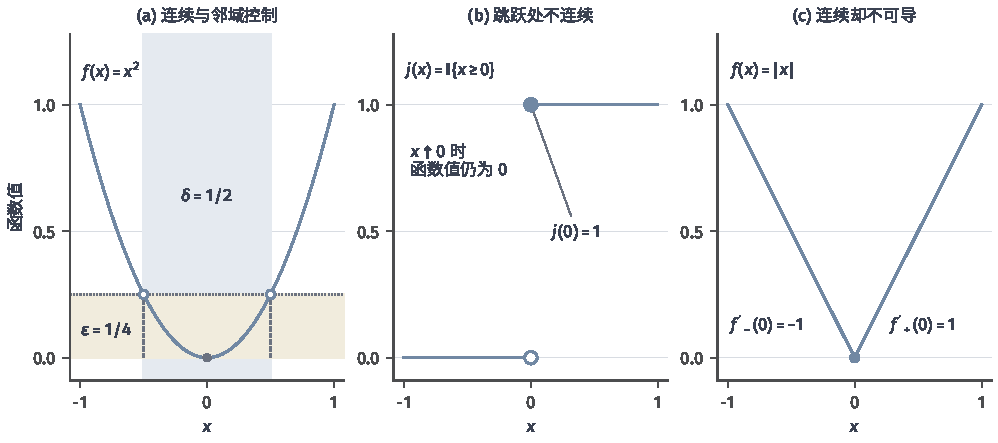
\includegraphics[width=169.0mm]{figures/01-mathematical-preliminaries-upper/01-mathematical-language-combinatorics-analysis-optimization/matplotlib/analysis-continuity-counterexamples/figure.pdf}
 \caption{平方函数、绝对值函数与阶跃函数在原点的差别。平方函数连续且可微；绝对值函数连续，但左右导数不同；阶跃函数的左右极限不同。连续性控制函数值的极限，可微性还要求差商具有同一个有限极限。}
 \label{fig:analysis-continuity-counterexamples}
\end{figure*}

\subsubsection{连续可微函数}

可导以后，还可以要求导函数连续。若$f$在开区间$I$上可导且$f'$连续，称$f$连续可微，记为$f\in C^1(I)$。在闭区间上使用$C^1([a,b])$时，要求$f$在闭区间连续、内点可导，且$f'$连续延拓到两端；延拓值就是相应单侧导数。

连续可微是比可微更强的要求。令$f(0)=0$、$f(x)=x^2\sin(1/x)$（$x\neq0$）。原点差商为$h\sin(1/h)\to0$，所以$f'(0)=0$；非零位置的导数为$2x\sin(1/x)-\cos(1/x)$，将在求导规则中得到。取$x_n=1/(2\pi n)$，有$f'(x_n)=-1$，故$f'$在$0$处不连续。导数存在并没有要求邻近位置的导数也接近它。

\subsection{微分的运算法则}
\label{sec:analysis-scalar-chain-rules}

以下设$f,g$在所讨论点的开邻域有定义，并在该点可导。求导规则来自差商极限或式~\eqref{eq:analysis-scalar-first-order}的一阶展开。

\subsubsection{四则运算的求导}

\paragraph{和与数乘}
差商的加法与数乘直接给出$(f+g)'=f'+g'$、$(cf)'=cf'$，其中$c$为实常数。减法是$c=-1$的情形。

\paragraph{乘积法则}
将$f(a+h)$和$g(a+h)$分别展开，乘积中一次项为$f'(a)g(a)h+f(a)g'(a)h$，两个增量的乘积属于$O(h^2)$。因此
\begin{equation}
 \begin{aligned}
 (f+g)'(a)&=f'(a)+g'(a),\\
 (fg)'(a)&=f'(a)g(a)+f(a)g'(a).
 \end{aligned}
\label{eq:analysis-scalar-sum-product-rules}
\end{equation}

\paragraph{商法则}
若$g(a)\neq0$，连续性先保证$a$附近的分母不为零。整理差商得
\[
 \left(\frac fg\right)'(a)
 =\frac{f'(a)g(a)-f(a)g'(a)}{g(a)^2}.
\]
分母非零既保证函数有定义，也保证右侧公式有意义。

\subsubsection{复合函数求导}

复合函数的输入变化先经过内层，再传入外层；总的一阶变化需要联系这两个局部变化率。
若$f$在$a$处可导，$g$在$f(a)$处可导，且复合在$a$附近有定义，则
\begin{equation}
 (g\circ f)'(a)=g'(f(a))f'(a).
\label{eq:analysis-scalar-chain-rule}
\end{equation}
这称为\term{链式法则}（chain rule）。令$k=f(a+h)-f(a)=f'(a)h+o(|h|)$，则$k=O(|h|)$。把它代入$g(f(a)+k)=g(f(a))+g'(f(a))k+o(|k|)$，余项仍为$o(|h|)$，于是得到公式。$k=0$时取余项为零，这个证明也覆盖$f'(a)=0$的情形，无需除以可能为零的中间增量。

\subsubsection{反函数求导}
逆映射已经连续，现在进一步判断它何时可导，以及变化率怎样由原函数的变化率决定。
设$f:I\to J$在区间$I$上连续且严格单调，$J=f(I)$，其反函数为$g=f^{-1}$。第~\ref{sec:analysis-inverse-continuity}节已证明$g$连续，因此像点趋近时，反像也趋近。若$f$在内点$a$处可导且$f'(a)\neq0$，令$b=f(a)$、$h=g(b+k)-a$，则$k\to0$时$h\to0$，并且
\[
 \frac{g(b+k)-g(b)}k
 =\frac{h}{f(a+h)-f(a)}\longrightarrow\frac1{f'(a)}.
\]
因此$g'(b)=1/f'(a)$。这个公式也与复合恒等式$f(g(y))=y$的链式法则一致；先用差商证明$g$可导，避免在证明中预设它的可导性。条件是所用反函数区间内一一对应，且所讨论点的原函数导数非零。

\paragraph{微分形式的运算法则}
把导数系数作用于增量$h$，同一规则可以写成微分形式：
\[
 \begin{aligned}
 \mathrm d(fg)_a(h)&=g(a)\,\mathrm df_a(h)+f(a)\,\mathrm dg_a(h),\\
 \mathrm d(g\circ f)_a(h)&=\mathrm dg_{f(a)}\bigl(\mathrm df_a(h)\bigr).
 \end{aligned}
\]
复合式先计算中间增量的一阶近似，再把它代入外层微分。

\subsubsection{基本初等函数的导数}
\label{sec:analysis-elementary-derivatives}

四则运算和链式法则把复杂函数的求导归结为基本函数的导数。下面从差商说明常用公式的依据，并给出各自的定义域。

\paragraph{常数函数与整数幂函数}
常数函数$f(x)=c$的差商恒为零，所以$f'=0$；恒等函数$f(x)=x$的差商恒为$1$，所以$f'=1$。
对正整数$m$，把$x^m$看成$m$个恒等函数的乘积，反复使用乘法求导规则。
每一项只对一个因子求导，其余$m-1$个因子保留，于是
\[
 (x^m)'=\underbrace{x^{m-1}+\cdots+x^{m-1}}_{m\text{项}}=mx^{m-1}.
\]
$m=1$时导数为$1$；$m=0$即常数函数。
结合商法则，对负整数$m$在$x\neq0$处同样有$(x^m)'=mx^{m-1}$；正整数幂在整个实轴上使用这一公式。

\paragraph{正弦函数与余弦函数}
采用弧度制。由第~\ref{sec:analysis-function-limits}节的标准极限$\sin h/h\to1$，以及$\cos h-1=-2\sin^2(h/2)$，可得$(\cos h-1)/h\to0$。正弦加法公式于是给出
\[
 \frac{\sin(x+h)-\sin x}{h}
 =\sin x\frac{\cos h-1}{h}+\cos x\frac{\sin h}{h}
 \longrightarrow\cos x.
\]
余弦加法公式同理给出$(\cos x)'=-\sin x$。这两条导数公式在整个实轴成立；若使用角度制，公式还会多出单位换算系数。

\paragraph{指数函数}
自然指数函数满足$e^{x+h}=e^xe^h$。利用前面陈述的标准极限$(e^h-1)/h\to1$，得到
\[
 \frac{e^{x+h}-e^x}{h}=e^x\frac{e^h-1}{h}\longrightarrow e^x.
\]
因此$(e^x)'=e^x$在整个实轴成立。这一推导只使用指数乘法公式与该标准极限。

\paragraph{对数函数与实数幂函数}
前面已知$e^x$连续、严格递增，两端分别趋于$0$与$+\infty$。对任意$y>0$，先选两点使指数值分别小于和大于$y$，再用介值定理得到原像；严格递增保证该原像唯一。因此指数函数的值域恰为$(0,\infty)$，并有反函数。自然对数$\log x$（也记$\ln x$）就定义为这个反函数。指数导数处处非零，反函数求导给出$(\log x)'=1/x$，范围为$x>0$。若$a>0$且$a\neq1$，由$a^x=e^{x\log a}$和$\log_a x=(\log x)/(\log a)$，再用链式法则得到
\[
 (a^x)'=a^x\log a\quad(x\in\mathbb R),\qquad
 (\log_a x)'=\frac1{x\log a}\quad(x>0).
\]
对任意实数$\alpha$，在$x>0$上定义$x^\alpha=e^{\alpha\log x}$，同样得到$(x^\alpha)'=\alpha x^{\alpha-1}$。这并未对负数底数的任意实数次幂作定义。

\subsection{闭区间上可微函数的性质}

导数记录一点处的变化率；现在要把它与区间上的极值、端点变化以及两点之间的变化幅度联系起来。
涉及闭区间$[a,b]$的中值结论将分别要求函数在闭区间上连续、在开区间$(a,b)$内可导，不要求端点具有双侧导数。

\subsubsection{局部极值与驻点}

\paragraph{局部极值}
若只关心某个输入附近的变化，就应先把邻近范围的极值与整个定义域的最值分开。
若存在$r>0$，使定义域内所有满足$|x-c|<r$的点都有$f(x)\geq f(c)$，则$c$称为局部极小点；若$x\neq c$时均为严格不等式，则称为严格局部极小点。
反向不等式定义局部极大点。局部极值只比较某个邻域内的函数值，区别于整个定义域上的最值。

\paragraph{Fermat定理}
局部极值比较邻近函数值，导数则描述一阶变化；两侧差商的符号把这两种信息联系起来。
内点允许从两侧比较，下面说明这种比较对导数的约束。
\begin{theorem}[Fermat定理]
\label{thm:analysis-fermat}
设$a<b$，$f:[a,b]\to\mathbb R$，$c\in(a,b)$。若$f$在$c$处可导，且$c$为$f$的局部极小点或局部极大点，则
\begin{equation}
 f'(c)=0.
\label{eq:analysis-scalar-first-order-necessary}
\end{equation}
\end{theorem}
\begin{proof}
设$c$为局部极小点。充分小的$h$满足$f(c+h)-f(c)\geq0$，
故$h>0$时差商非负、$h<0$时差商非正。
两侧差商趋于同一个有限导数，因而同时有$f'(c)\geq0$与$f'(c)\leq0$，即$f'(c)=0$。
局部极大点对$-f$应用同一论证即可。
\end{proof}
导数为零的点称为\term{驻点}（stationary point），但驻点未必是极值点，例如$x^3$在$0$处。
边界极值也不要求导数为零：$x$在$[0,1]$的最小点为$0$，右导数却为$1$；这里缺少Fermat定理要求的内点条件。

\paragraph{一阶导数判别法}
驻点条件本身不能判定极值，还需考察函数在驻点两侧的变化方向。
下面先给出符号判据，其依据将在后面的单调性小节中证明。
\begin{theorem}[一阶导数判别法]
\label{thm:analysis-first-derivative-test}
设$r>0$，$f$在$[c-r,c+r]$上连续、在$(c-r,c+r)$内可导，且$f'(c)=0$。
若
\[
 f'(x)<0\quad(c-r<x<c),\qquad
 f'(x)>0\quad(c<x<c+r),
\]
则$c$为$f$的严格局部极小点。
若两个区间上的导数符号分别为正和负，则$c$为$f$的严格局部极大点。
\end{theorem}
第一种符号变化对应先降后升，第二种对应先升后降。
仅有$f'(c)=0$不够；接下来先建立中值定理，再由它证明导数符号确实控制区间内的增减，最后补出这一判别法的证明。

\subsubsection{中值定理}

\paragraph{Rolle定理}
当函数两端取同一值时，整体净变化为零。
下面说明连续、可导条件如何保证内部有一处瞬时变化率也为零。
\begin{theorem}[Rolle定理]
\label{thm:analysis-rolle}
设$a<b$，$f:[a,b]\to\mathbb R$在$[a,b]$上连续、在$(a,b)$内可导。
若$f(a)=f(b)$，则
\[
 \exists c\in(a,b),\qquad f'(c)=0.
\]
\end{theorem}
\begin{proof}
若$f$恒定，任取$c\in(a,b)$即可。
否则存在$x_0\in(a,b)$使$f(x_0)\neq f(a)$。
由闭区间上的极值定理，$f$达到最大值和最小值；若$f(x_0)>f(a)=f(b)$，最大值必在内点达到，
若$f(x_0)<f(a)=f(b)$，最小值必在内点达到。
在所选内点应用Fermat定理，得到导数为零。
\end{proof}

\paragraph{Lagrange中值定理}
两端取值不同时，可以先减去连接两个端点的直线，使剩余函数两端相等。
Rolle定理由此把整段平均变化率与某个内点的瞬时变化率联系起来。
\begin{theorem}[Lagrange中值定理]
\label{thm:analysis-lagrange-mean-value}
设$a<b$，$f:[a,b]\to\mathbb R$在$[a,b]$上连续、在$(a,b)$内可导，则存在$c\in(a,b)$使
\begin{equation}
 f(b)-f(a)=f'(c)(b-a).
\label{eq:analysis-mean-value-theorem}
\end{equation}
等价地，$f'(c)=[f(b)-f(a)]/(b-a)$。
\end{theorem}
\begin{proof}
令
\[
 H(x)=f(x)-f(a)-\frac{f(b)-f(a)}{b-a}(x-a).
\]
$H$在$[a,b]$上连续、在$(a,b)$内可导，并满足$H(a)=H(b)=0$。
Rolle定理给出某个$c\in(a,b)$使
$H'(c)=f'(c)-[f(b)-f(a)]/(b-a)=0$，整理即得结论。
\end{proof}
这就是Lagrange\term{中值定理}（mean value theorem）的含义：区间上的平均变化率等于某个内点的瞬时变化率。
定理不要求导函数连续，只要求函数在每个内点可导。


图~\ref{fig:analysis-process-mean-value-parallel}说明中值定理将两个端点之间的平均变化率，联系到区间内部某一点的瞬时变化率。
\begin{figure}[!htbp]
 \centering
 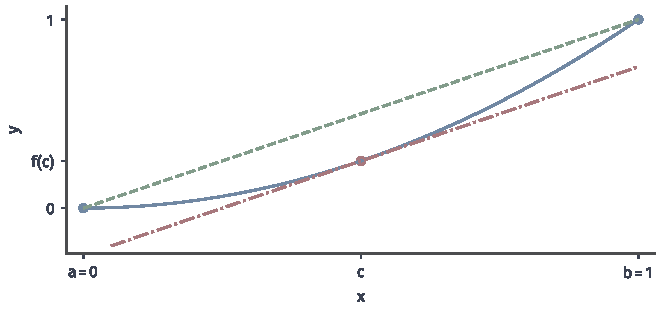
\includegraphics[width=112.0mm]{figures/01-mathematical-preliminaries-upper/01-mathematical-language-combinatorics-analysis-optimization/matplotlib/chapter3-concept-processes/mean-value-parallel.pdf}
 \caption{$f(x)=x^2$在$[0,1]$上，绿虚线为端点割线，红点划线为$c=1/2$处的切线。两线平行，因为$f'(c)=1=[f(1)-f(0)]/(1-0)$。图中切线与割线高度不同；相等的是斜率，而不是两条直线。}
 \label{fig:analysis-process-mean-value-parallel}
\end{figure}

\paragraph{Cauchy中值定理}
同时观察两个函数时，可以把它们的端点增量放进同一个辅助函数，从而联系这两种变化。
采用交叉相乘的形式，可以先得到不依赖分母非零的结论。
\begin{theorem}[Cauchy中值定理]
\label{thm:analysis-cauchy-mean-value}
设$a<b$，$f,g:[a,b]\to\mathbb R$均在$[a,b]$上连续、在$(a,b)$内可导，则存在$c\in(a,b)$使
\[
 (f(b)-f(a))g'(c)=(g(b)-g(a))f'(c).
\]
若进一步有$g'(x)\neq0$对每个$x\in(a,b)$成立，则$g(b)\neq g(a)$，并可写为
\[
 \frac{f(b)-f(a)}{g(b)-g(a)}=\frac{f'(c)}{g'(c)}.
\]
\end{theorem}
\begin{proof}
令
\[
 \begin{aligned}
 H(x)={}&(f(b)-f(a))(g(x)-g(a))\\
        &-(g(b)-g(a))(f(x)-f(a)).
 \end{aligned}
\]
$H$继承两函数的连续、可导条件，并有$H(a)=H(b)=0$。
应用Rolle定理得$H'(c)=0$，展开导数即为交叉相乘形式。
若$g'$处处非零，$g(b)=g(a)$会由Rolle定理推出某个内点$g'=0$，产生矛盾，故端点增量非零。
所选点的$g'(c)$也非零，此时才能除法得到比值形式。
\end{proof}
取$g(x)=x$时，Cauchy中值定理回到Lagrange中值定理。

\subsubsection{单调性}

中值定理把任意两点的函数增量写成一个内点导数乘以输入增量，因此导数符号可以控制整段的增减。
关键是任意两点之间的整段都属于定义域。
\begin{theorem}[导数符号与单调性]
\label{thm:analysis-derivative-monotonicity}
设$a<b$，$f:[a,b]\to\mathbb R$在$[a,b]$上连续、在$(a,b)$内可导。
若$f'(x)\geq0$对所有$x\in(a,b)$成立，则$f$在$[a,b]$上单调不减；若处处有$f'(x)>0$，则严格递增。
相应地，$f'\leq0$蕴含单调不增，$f'<0$蕴含严格递减。
若$f'$在$(a,b)$内恒为零，则$f$在$[a,b]$上为常数。
\end{theorem}
\begin{proof}
任取$a\leq x<y\leq b$，在$[x,y]$上应用Lagrange中值定理，存在$\xi\in(x,y)$使
\[
 f(y)-f(x)=f'(\xi)(y-x).
\]
因为$y-x>0$，右侧的符号由$f'(\xi)$决定，于是得到四种单调性结论。
导数恒为零时，任意两点的函数值都相等，所以函数为常数。
\end{proof}
导数恒零只保证每个区间上为常数。若定义域由分离的区间组成，各段的常数未必相同，不能跨过定义域的缺口使用中值定理。

现在可以补出定理~\ref{thm:analysis-first-derivative-test}的证明：导数的两侧符号分别控制了驻点与任意邻近点之间的变化。
\begin{proof}[一阶导数判别法的证明]
先考虑左负右正的情形。对$c-r<x<c$，在$[x,c]$上应用单调性定理得$f(x)>f(c)$；
对$c<x<c+r$，在$[c,x]$上应用同一定理也得$f(x)>f(c)$。
所以$c$两侧充分近的异点都有更大的函数值，$c$为严格局部极小点。
左正右负时反向比较，得到$f(x)<f(c)$，因此$c$为严格局部极大点。
\end{proof}
导数为零并非严格单调的障碍：例如$x^3$在整个实轴严格递增，但在$0$处导数为零。
因此“导数处处严格为正”是严格递增的充分条件，不能当作必要条件。

\subsubsection{Lipschitz条件}

导数的符号控制增减方向；若还能统一限制导数的绝对值，就可以控制任意两点之间的变化幅度。
中值定理把这一导数上界直接转为前面定义的Lipschitz条件。
\begin{theorem}[有界导数与Lipschitz条件]
\label{thm:analysis-bounded-derivative-lipschitz}
设$a<b$，$f:[a,b]\to\mathbb R$在$[a,b]$上连续、在$(a,b)$内可导。
若存在有限常数$L\geq0$使$|f'(x)|\leq L$对所有$x\in(a,b)$成立，则
\[
 \forall x,y\in[a,b],\qquad |f(y)-f(x)|\leq L|y-x|.
\]
即$f$在$[a,b]$上为Lipschitz连续函数，$L$是一个Lipschitz常数。
\end{theorem}
\begin{proof}
$x=y$时两侧都为零；$x<y$时，Lagrange中值定理给出$\xi\in(x,y)$，使
\[
 |f(y)-f(x)|=|f'(\xi)|\,|y-x|\leq L|y-x|.
\]
$x>y$时交换两点即可。
\end{proof}
例如$f(x)=x^2$在$[0,1]$内有$|f'(x)|=2x\leq2$，所以可以取$L=2$，与前面的直接估计一致。
这一结论仍要求两点间的整段都在定义域中；它给出的是可导函数满足Lipschitz条件的充分保证。

若$f\in C^1([a,b])$，连续导数在闭区间上有界，因而由上述定理得到Lipschitz连续，再由连续性条件的关系得到绝对连续和一致连续。
这些结论的逆向不能保证导数处处存在：$|x|$在$[-1,1]$上Lipschitz连续，却在$0$处不可导。
控制函数值变化与要求经典导数处处存在，因而是两种需要分别检查的条件。

\subsection{高阶微分}

\subsubsection{高阶导数}

\paragraph{二阶导数}
要研究斜率本身怎样变化，可以继续对导函数求导。
导函数$f'$若还可导，其导数称为二阶导数，记为$f''$。

\paragraph{高阶导数}
依次定义$f^{(r)}=(f^{(r-1)})'$，并约定$f^{(0)}=f$。
若直到第$r$阶导数都存在且连续，称$f$为$r$阶连续可微函数，记为$f\in C^r$。$C^r([a,b])$的端点导数采用从内部取得的连续延拓，与前面$C^1$的约定相同。

在以$x$为独立变量的记号中，$r$阶微分写作$\mathrm d^rf=f^{(r)}(x)(\mathrm dx)^r$；它给出高阶变化的系数，近似实际增量时还需Taylor系数与余项。

\subsubsection{二阶近似}
\label{sec:analysis-second-order-curvature}
对$f(x)=x^3-3x$，$f''(x)=6x$，所以$f''(1/2)=3$。加入二次项后，式~\eqref{eq:analysis-cubic-linear-model}成为
\begin{equation}
 T_2(h)=-\frac{11}{8}-\frac94h+\frac32h^2.
\label{eq:analysis-cubic-quadratic-model}
\end{equation}
$h=0.1$时，$T_2=-1.585$，与实际值$-1.584$相差$0.001$。正的二阶导数说明斜率随$x$增加，曲线在这一邻域内向上弯；二次项正好补充切线近似遗漏的这一部分变化。图~\ref{fig:analysis-derivative-orders}比较了两阶近似及其余项。

\subsubsection{Taylor公式}
\label{sec:analysis-taylor-approximation}

\paragraph{Lagrange余项}
要把上面的近似推广到任意阶，需要同时控制截去的误差。设$r\geq0$为整数，$f$在连接$x_0$与$x_0+h$的线段的开邻域内属于$C^{r+1}$。若$h\neq0$，则两端之间存在$\xi$使
\begin{equation}
 f(x_0+h)=\sum_{k=0}^r\frac{f^{(k)}(x_0)}{k!}h^k
 +\frac{f^{(r+1)}(\xi)}{(r+1)!}h^{r+1}.
\label{eq:analysis-taylor-arbitrary-order}
\end{equation}
\begin{proof}
记$T_r(t)=\sum_{k=0}^rf^{(k)}(x_0)(t-x_0)^k/k!$，$R=f(x_0+h)-T_r(x_0+h)$。令
\[
 H(t)=f(t)-T_r(t)-R\frac{(t-x_0)^{r+1}}{h^{r+1}}.
\]
$H$在两端为零，且$r\geq1$时$H'(x_0),\ldots,H^{(r)}(x_0)$均为零。第一次用Rolle定理得到两端之间的零导数点，再把该点与$x_0$的零导数条件结合，逐次使用Rolle定理。共用$r+1$次后得到某个中间点$\xi$满足
\[
 0=H^{(r+1)}(\xi)=f^{(r+1)}(\xi)-\frac{(r+1)!}{h^{r+1}}R.
\]
整理即得公式。$r=0$时只用一次Rolle定理；$h<0$时交换区间左右端点，论证相同。
\end{proof}
若该线段上$|f^{(r+1)}|\leq M$，余项的绝对值不超过$M|h|^{r+1}/(r+1)!$。因此近似的精度既与阶数有关，也与位移大小及导数界有关。第~\ref{sec:analysis-integration-remainders}节还将给出积分余项，本处的证明不依赖积分。

对立方函数，完整展开为
\[
 f(1/2+h)=-\frac{11}{8}-\frac94h+\frac32h^2+h^3.
\]
线性近似遗漏$3h^2/2+h^3$，二次近似只遗漏$h^3$；四阶及以上导数全为零，三阶展开已经精确。
\begin{figure*}[htbp]
 \centering
 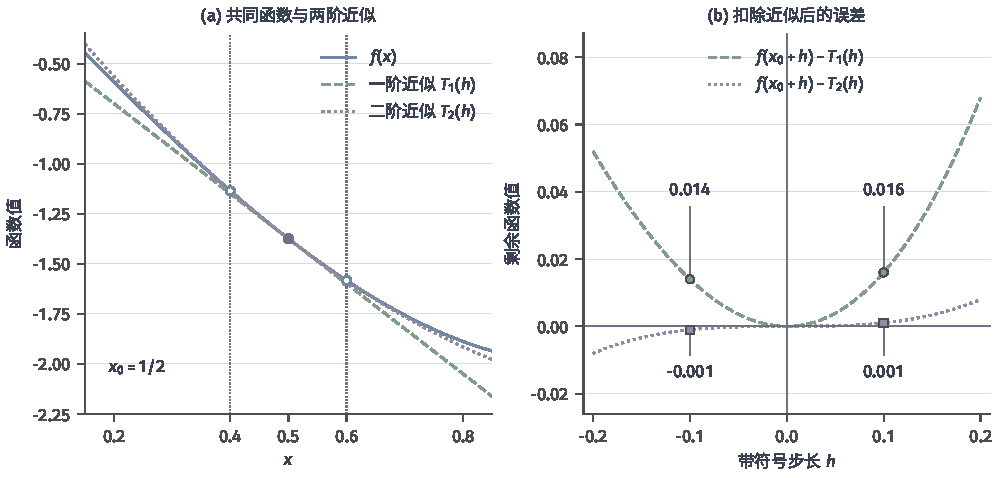
\includegraphics[width=169.0mm]{figures/01-mathematical-preliminaries-upper/01-mathematical-language-combinatorics-analysis-optimization/matplotlib/analysis-derivative-orders/figure.pdf}
 \caption{$f(x)=x^3-3x$在$x_0=1/2$处的Taylor近似，$h=x-x_0$。左图比较原函数、切线近似$T_1$与二次近似$T_2$；右图给出相应的带符号余项$3h^2/2+h^3$和$h^3$。标记点对应$h=\pm0.1$，余项的正负说明真值位于近似值的哪一侧。}
 \label{fig:analysis-derivative-orders}
\end{figure*}

\paragraph{Peano余项}
如果只关心位移趋零时的误差阶，可以不保留中间点，改用小量记号描述余项。
若$f\in C^r$、$r\geq1$，则在$x_0$附近有
\[
 f(x_0+h)=\sum_{k=0}^r\frac{f^{(k)}(x_0)}{k!}h^k+o(|h|^r).
\]
对$r-1$次Taylor公式使用Lagrange余项，再从$f^{(r)}(\xi_h)h^r/r!$中减去$f^{(r)}(x_0)h^r/r!$。因为$\xi_h\to x_0$且$f^{(r)}$连续，差除以$|h|^r$趋零，就得到这一形式。它描述局部误差的阶；若需要有限位移下的具体界，可使用上面的Lagrange余项估计。

\paragraph{二阶导数判别法}
在驻点处，一阶项为零；二阶Taylor公式把局部增减进一步联系到二阶导数的符号。
设$f$在驻点$a$附近属于$C^2$。Taylor公式给出$f(a+h)-f(a)=\tfrac12f''(\xi_h)h^2$。若$f''(a)>0$，连续性使充分近的$f''(\xi_h)\geq f''(a)/2$，因而非零小增量使函数值严格增加，$a$为严格局部极小点；$f''(a)<0$时为严格局部极大点。反之，在上述$C^2$条件下，局部极小点必须有$f''(a)\geq0$，局部极大点必须有$f''(a)\leq0$。

$f''(a)=0$时该判别法没有结论：$x^4$、$-x^4$在$0$处分别有严格局部极小值和极大值，$x^3$则没有极值，三者在原点的前两阶导数都为零。

\FloatBarrier
